\section{Methodology}
The research methodology is summarized by the diagram given in Figure \ref{methodology-new}. The primary purpose of this research is to assess the  effect of dietary patterns on the ACR levels, survival and morbidity for chronic kidney disease (CKD)/End Stage Renal Disease (ESRD) patients.

\begin{figure}
\centering
%\begin{center}
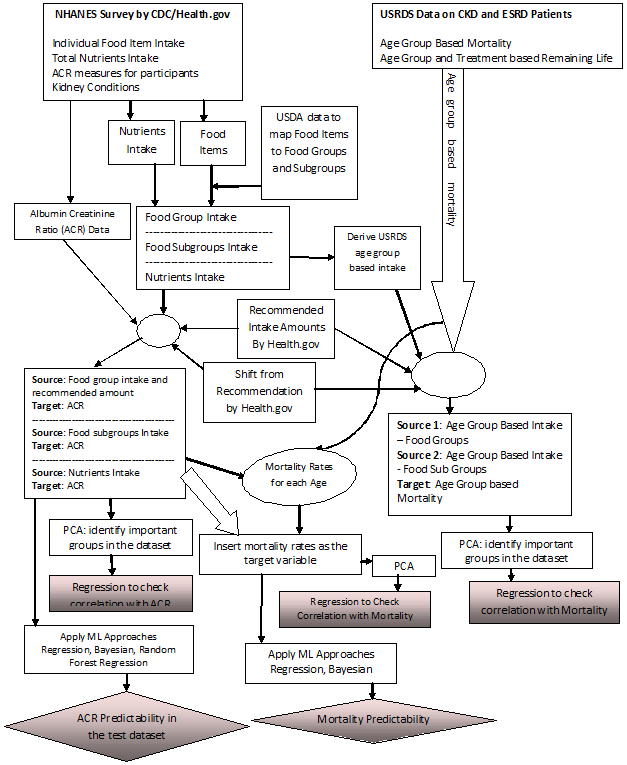
\includegraphics[scale=0.48]{methodologies-enhanced}
%\end{center}
\caption{\textbf{Methodology in a Diagram}}
\label{methodology-new}
\end{figure}

\subsection{Methodology Overview}
\noindent  A dataset released by CDC/Health.gov with the dietary habits and ACR values for 10,000 individuals are studied. Also, age group based mortality and survival of CKD/ESRD patients provided by USRDS are studied. Afterwards, utilized Principal Component Analysis to identify the most important food groups and subgroups affecting the ACR value and the Mortality/Survival.  Statistical regression and factor analysis was then applied to understand the correlation between ACR, and Mortality/Survival to dietary patterns. Machine learning approaches including Regression, Polynomial Regression, and Bayesian with or without 10 fold cross validations are applied on the datasets to understand if dietary patterns can be used to predict ACR values and mortality. 

\noindent 
In addition to studying the association of CKD mortality and ACR values with ratios from the recommended high, we have explored the potential impact of diet recommendation shift [11], on the incidence of CKD in the general population.

\subsection{Study Selection}
%\noindent \textbf{Study Selection}

\medskip 

\noindent For dietary patterns, CKD measures (such as Albumin to Creatinine Ratio - ACR), and Kidney condition measures, a dataset from the National Health and Nutrition Examination Survey on dietary habits conducted by the CDC [10] was used. The survey has data from 1996 to 2016 [10]. This study primarily utilized data for 2015-2016. The survey recorded 24 hours individual food item intake amount. Two surveys were taken within 3 to 10 days apart. Each survey provided food item intake amounts in a day and recorded the diet style as well as diet-restrictions. Individual food items are represented using USDA food code. The survey also provided total nutrients data. CDC also released examination, laboratory, demographics, and other related data for those participants. This study explored and utilized examination data such as Kidney Condition data, laboratory data such as ACR data \& Blood Pressure data, and demographics data for age.

\medskip 
\noindent For mortality and survival information, dataset from the United States Renal Data System (USRDS) on CKD and ESRD [16, 17] were utilized. “USRDS investigates the transition of care from CKD to ESRD and end-of-life care for those with advanced kidney disease” [19]. USRDS also releases data on the Incidence, Prevalence, Patient Characteristics, and Treatment Modalities on CKD, and ESRD patients. USRDS  reports survival and mortality using metrics such as Mortality rates, Total Mortality Count,  90 day survival for dialysis and/or transplantation patients,  10 year survival for dialysis and/or transplantation patients, Average Expected remaining lifetime with or without pre-condition and treatment options used.  The data are either aggregated or patient specific detail data. However, only aggregated data are public where patient specific data access requires special request and permission. This research utilized only the public dataset i.e. age-group based aggregated data. In couple of experiments, aggregated age-group based data from USRDS was mapped to specific age for NHANES data for each age and participants.

\medskip
\noindent The dietary survey data (NHANES) represented the food items taken by the participants using USDA food codes [14, 12, 13]. Hence, USDA food codes [14, 12, 13] are used to assign food groups and subgroups to the NHANES [10] survey data to properly group/subgroup the dietary intake of the participants with some customizations.

\subsection{Data Synthesis}
\noindent NHANES survey data as provided for two days are averaged to get the intake amount for one day. Both individual food item data and nutrients intake data are averaged. USDA food codes are used to map food items to food groups and subgroups.

\noindent ACR and Kidney condition data for each individual are merged with the averaged food groups, subgroups, and nutrients data. This data was further complemented with the food group recommendations data from health.gov, and mortality rate by age from the USRDS. ACR values and mortality rate  are used as the target variables.

\noindent PCA was applied to find out important food groups and subgroups while regression was applied to find potential associations with ACR and Mortality. Linear Regression, Polynomial Regression, Random Forest Regression, Bayesian prediction with or without 10 fold cross validations were applied to study the predictability of ACR Values and Mortality in the test dataset. 

\noindent In another mortality experiment, the above synthesized datasets were aggregated for USRDS age  groups to calculate average food group/subgroup intake by age groups. 